\section{提案システム}
本章では,DNSトンネリングの発生抑止を目的に設計した名前解決システムDNS-TD(DNS for Tunneling Deterrence)を説明する.
\begin{figure}[h]
 \centering
 \label{fig:abstruct-DNS-TD-architecture}
 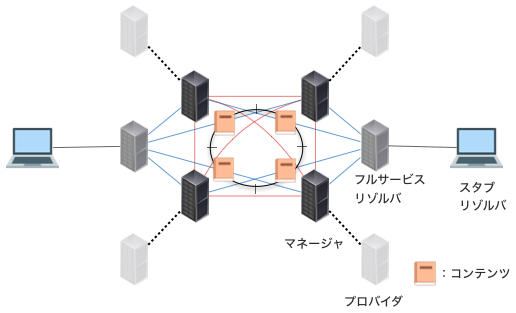
\includegraphics[scale=0.6]{figure/new-architecture-DNS-TD.png}
 \caption{提案システムの概略図}
\end{figure}
\subsection{概要}
\label{sec:DNS-TD}
現在のDNSの名前解決の仕組みにおいて,名前空間が委譲の仕組みに基づきドメインごとにゾーンで分割されているため,名前解決クエリは目的ドメインの権威サーバまで転送される必要がある.
また,リソースレコードはドメイン名に関係ない任意の情報を関連づけることができる設計になっている.
この2つの特性に起因して,DNSトンネリングは機能する.
すなわち,再帰問い合わせに基づく名前解決の仕組みとドメイン名に関連づけるレコード情報に高い自由度を排除することによって,DNSトンネリングの発生抑止を実現することができる.
一方で,名前解決システムとしての機能を維持するために,以下に示す2つの性質を満たす必要がある.
\begin{description}
 \item[名前解決]\mbox{}\\ ドメイン名にIPアドレスなどの情報を関連づけることができ,それを解決することができる
 \item[スケーラビリティ]\mbox{}\\ ドメイン名の増加および関連づけられるレコード情報の増加に対応することができる
\end{description}
%%設計要件
以上から,期待される名前解決システムの要件は,上記2つの性質を満たしながら先の特性を排除することである.
そこで,提案システムDNS-TDでは,不足が無視できる程度に大規模の名前空間と範囲に基づくゾーン分割によって名前解決とスケーラビリティを実現し,再帰問い合わせの特性を排除させ,認証システムによってリソースレコードの自由度を下げることで上記の要件を満たす.
以降では,その要件を満たすための手法および仕組みを概観する.\newline

\textbf{不足が無視できる程度に大規模の名前空間}\\
DNS-TDは,ドメイン名とレコード情報の組みには識別子を付与され,この識別子は672bit(84bytes)の有限名前空間上の一意に写像されたものを使用する.
識別子は,ドメイン名とそのレコードタイプの文字列和をメッセージとするハッシュ関数から算出されるダイジェストである.
例えば,ドメイン名が``www.example.com"でレコードタイプが``A"のペアを考える.
この場合,メッセージが``www.example.comA",識別子がこのメッセージをハッシュ関数に与えたダイジェスト``例:86ff(...中略...)8485"となる.\newline

\textbf{範囲に基づくゾーン分割}\\
識別子の名前空間について,ソートされた空間の特定範囲に基づいてゾーンが分割される.
提案システムにおけるサーバは,このようにして分割されたゾーンをそれぞれ担当することによって,分散的な管理システムとして協調することで名前解決機能を実現する.
提案システムにおけるサーバ機能は,一部を除いた\footnote{ccTLDとブランドTLDはSLDとして扱われ,それぞれ``cc"と``brand"というTLDに接続される.}gTLDによって集約される.
すなわち,SLD以降の権威サーバにサーバ機能はなく,ドメイン名とレコードタイプの作成と更新の機能のみを担う.
既存のSLD以降の権威サーバは,gTLDサーバにドメイン名の階層構造の序列を維持した状態で連結し,コンテンツ情報の操作を通じてgTLDにサーバ機能を委任する.
このように既存システムの権威サーバの機能を,サーバ機能とコンテンツ作成などの操作機能に分類することによって,クライアントからの権威サーバへの透過性を防ぎ,DNS Exfiltrationを抑止する.\newline

\textbf{認証システム}\\
DNS-TDでは,認証の仕組みを導入することでレコード情報の真正性を確保する設計をとっている.
既存システムでは,ドメイン名に関連づける情報はゾーンファイルにて定義されるが,ゾーンファイルを編集する主体が権威サーバであるため任意の情報を含めることができる設計になっている.
提案システムでは,先に述べるようにコンテンツの管理機能と編集機能とを分離させる.
コンテンツの編集機能は,サーバに階層的に接続されるノード,プロバイダが担う.
プロバイダを起点として行われるコンテンツへの操作は,認証機関を介在した後でサーバで実行される設計になっている.
この認証プロセスでは,依頼者(プロバイダ)情報およびレコード情報とその関連先となるドメイン名について真正性について検証される.
例えば,アドレスなどの情報であれば接続性が検証され,その他の情報であればレコード情報をドメイン名に関連づける正当性などが検証される.
この認証プロセスをパスし,証明書が発行されたコンテンツのみが,サーバによって管理される.
この認証プロセスによって,不審な情報がドメイン名に関連づけられることを未然に対処する.

以降では,上記3つのアプローチについて詳細に説明する.
また,DNS-TDで使う用語を表~\ref{tab:refres-terminology}にてまとめて示す.
\begin{table}[h]
 \centering
  \begin{tabular}{cl}
    \toprule
    \multicolumn{1}{c}{\textbf{表記}} & \multicolumn{1}{c}{\textbf{意味もしくは機能}}\\
    \midrule

    コンテンツ & \begin{tabular}{l}・識別子に関連づけられたレコード情報の実体\end{tabular}\\ \hline

    コンテンツID & \begin{tabular}{l}・識別子\end{tabular}\\ \hline

    レコード情報 &
      \begin{tabular}{l}
        ・リソースレコードの具体的な値\\
        (E.g. IPアドレス)
      \end{tabular}\\ \hline

     リソースレコードタイプ &
      \begin{tabular}{l}
        ・オブジェクトに関連づけるリソースレコードの型\\
        (E.g. A, AAAA, MX)
      \end{tabular}\\ \hline

    オブジェクト &
      \begin{tabular}{l}
       ・問い合わせる対象\\
       (E.g. ドメイン名もしくはIPアドレス)
      \end{tabular}\\ \hline

    スタブリゾル & \begin{tabular}{l}・名前解決クライアント\end{tabular}\\ \hline

    フルサービスリゾルバ &
      \begin{tabular}{l}
       ・スタブリゾルバからのクエリハンドリング\\
       ・識別子の作成
      \end{tabular}\\ \hline

    マネージャ &
      \begin{tabular}{l}
       ・フルサービスリゾルバからのクエリハンドリング\\
       ・ゾーンの管理\\
       ・コンテンツの保持
      \end{tabular}\\ \hline

    プロバイダ & \begin{tabular}{l}・コンテンツの作成・更新・削除操作\end{tabular}\\

    \bottomrule
  \end{tabular}
 \label{tab:refres-terminology}
 \caption{SORESにおける用語}
\end{table}



\newpage
\subsection{システムアーキテクチャ}
\label{sec:system-architecture}
本節では,DNS-TDのシステムアーキテクチャについて説明する.
現在,DNSはインターネットの根幹に位置づく技術であり,ほぼ全てのクライアントノードは既存システムが提供するアーキテクチャおよびプロトコルに依存している背景がある.
このため,システムのアーキテクチャの再構成において,エッジノードに対して変更が加えられるのは,導入負荷が高くなることが予想される.
現在のDNSによる名前解決は,フルサービスリゾルバを介在させながら,スタブリゾルバをクライアント,権威サーバをサーバとするクライアントサーバアーキテクチャで構成されている.
DNS-TDでは,導入フェーズで予想されるクライアントに対する名前解決処理システムの負荷を軽減することを目的として,従来同様のクライアントサーバアーキテクチャを踏襲する.
サーバ群は,図~\ref{fig:system-architecture}で示すように,相互で接続されたフルメッシュなネットワークで構築される.
\begin{figure}[htbp]
 \centering
 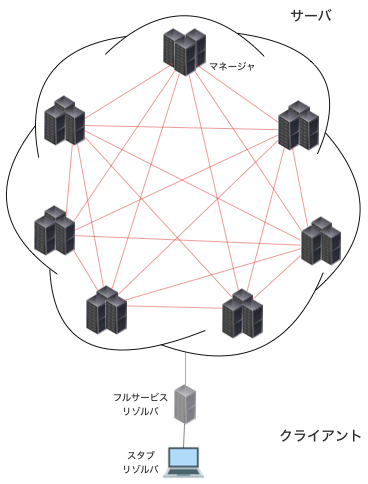
\includegraphics[scale=0.5]{figure/system-architecture.png}
 \caption{DNS-TDにおけるクライアントサーバアーキテクチャ}
 \label{fig:system-architecture}
\end{figure}
%クライアントからクエリは,フルサービスリゾルバを経由したのち
%コンテンツは,そのコンテンツIDとそのマネージャのゾーンを対応づけた対応表に基づいて一意に担当する
%各サーバは,コンテンツをそのコンテンツIDに基づいて分散的にかんりする
%クライアントからのクエリがあった際には
%コンテンツを分散的に管理しクライアントからのクエリに応答する.
%DNS-TDにおけるドメイン名の名前空間も既存システム同様に階層的な構造で構成されるが,サーバ

\subsection{サービスノード}
本節では,DNS-TDにおける各サービスノードの機能と他のサービスとの関わりについて詳細に説明する.
DNS-TDの名前解決ネットワークにおいて,クライアントがスタブリゾルバ,サーバの機能はマネージャが担当する.\newline

\hspace{-12pt}\textbf{スタブリゾルバ}\\
\label{sec:stab-resolver}
\hspace{12pt}スタブリゾルバは,既存システムと変わらない.
これは第~\ref{sec:system-architecture}節で述べるように,名前解決の仕組みの変化に伴ってクライアントに接続障害が発生する可能性がある.
既存のDNSに依存したクライアントの存在を踏まえて,接続性に影響を与えないためにスタブリゾルバは現行通りの方法で目的のリソース情報を解決することができる設計になっている.
すなわち,スタブリゾルバは,IPアドレスをはじめとしたオブジェクトに関連づけられたレコード情報を問い合わせ,目的サービスを提供するサーバのリソースにアクセスするクライアントノードである.
既存システム同様,スタブリゾルバのクエリはフルサービスリゾルバに転送され,キャッシュにヒットした場合には即座にレコード情報の応答結果を取得する.
ヒットしなかった場合には,フルサービスリゾルバがスタブリゾルバに変わって,サーバにクエリを転送し,応答結果をスタブリゾルバに返す.\newline

\hspace{-12pt}\textbf{マネージャ}\\
%具体的なTLDについてしっかりこのセクションで説明するべき
%マネージャの数
%プロバイダからの応答について説明するべきか
\hspace{12pt} マネージャは,2つの機能を担うサービスノードである.
それは,クライアントからの問い合わせに応答する機能と他のマネージャに操作リクエストを転送する機能である.
マネージャは,既存システムにおける権威サーバから分離した機能の一部であり,その残りの機能はプロバイダが担当している.
はじめに,マネージャとドメインおよびプロバイダの関係について説明する.

DNS-TDでは,既存のドメインの階層構造は引き継がれ,マネージャ・プロバイダそれぞれが独自のドメインを持っている.
プロバイダは,マネージャと親子関係にあるノードであり,マネージャが上位ドメイン,プロバイダが下位ドメインという構成である.
マネージャは,既存システムにおけるTLDに相当するドメインを保持する.
現在,TLDには国や地域に割り当てられるccTLDと分野別のgTLDの2つに大別することができる.
DNS-TDでは,コンテンツはそのIDに基づき管理する主体が決定する.
このため,ccTLDがマネージャである場合,国家間が抱えるナショナリズムや政治に起因して,名前解決システムの全体の運用に支障を来す事態が発生する可能性がある.
このことを回避するために,DNS-TDの設計ではマネージャが保有できるTLDをgTLDに限定している.
ccTLDは,``country"をドメインに持つマネージャにサーバ機能を委譲し,プロバイダとしてレコード情報の操作を行うことで現在のTLDと同等の位置づけを保つ.
これは,ドメインが``jp.country"となるのではなく,サーバ機能を``country"をドメインに持つマネージャに委ねるということである.
他方で現在,gTLDにはコミュニティ以外に``google"をはじめとした企業TLDがある.
先の国や地域に基づくシナリオであったように,民間企業の勝手な判断でインターネット全体に影響が波及するような接続性の断絶は起きうる.
そこで,企業やブランドを表すTLDは,``brand"というドメインにもつマネージャにサーバ機能を委譲し,プロバイダとして存在を継続させる.
その他のクラスとして分類することが困難な``foo"といったTLDについては,``misc"というドメインを持つマネージャにサーバ機能を委譲させる.
このように,DNS-TDでは,ドメインの名前空間を継続しながら,サーバとしての機能を再定義する.

以上のことを踏まえて,マネージャの機能について説明する.
1つ目は,ドメイン名とそれに関連づけられたレコード情報を保持し,フルサービスリゾルバからの問い合わせに応答する機能である.
マネージャは,レコード情報を管理するためにデータベースを用いる.
マネージャが保持するコンテンツは,そのドメイン名とレコードタイプによって決まる.
必ずしも自身のドメインを含むコンテンツを保持するわけではない.
例えば,``www.example.com"のAレコードについて考える.
この組のコンテンツIDが``47d8(中略\footnote{224bitのハッシュ値を表す.})cb6"であるとする.
他方で,``com"マネージャのゾーンは,``a000(中略)000"から``bzzz(中略)zzz"を担当しているとする.
また,``org"マネージャが``4000(中略)000"から``5zzz(中略)zzz"を担当しているとする.
この時,``www.example.com"はcomというTLDをもつが``com"マネージャではなく,``org"マネージャが保持する.
このようにして,コンテンツの管理は,ドメインに基づいて管理されるのではなくコンテンツIDの値とハッシュ値の範囲に基づいて決まる.

\begin{table}[htb]
 \caption{マネージャが使用する関数と保持する情報}
 \centering
  \begin{tabular}{ll}
    \toprule
		\multicolumn{1}{c}{\textbf{表記}} & \multicolumn{1}{c}{\textbf{意味}} \\
    \midrule
		parser() & クエリパケットをデータ構造に分解する関数 \\
		db\_accesser() & データベースにクエリする関数 \\
		benigh\_responce() & 正常応答用のペイロードを作成する関数 \\
		error\_responce() & 不在応答用のペイロードを作成する関数 \\
		payload.pack() & パケットのDNSのデータ構造にパックする関数 \\
		sendto() & クライアントに結果を応答する関数 \\
		record\_value & レコード情報 \\
    \bottomrule
  \end{tabular}
 \label{tab:discription-manager}
\end{table}

\begin{algorithm}[htbp]
 \caption{マネージャにおける名前解決問い合わせ処理}
 \label{algo:query-process}
  \SetKwProg{Fn}{}{\string:}{}
  \SetKwFunction{Handler}{handler}
  \SetKwFunction{Parse}{parser}
  \SetKwFunction{Database}{db\_accesser}
  \SetKwFunction{Noerror}{generate\_packet}
  \SetKwFunction{Error}{generate\_errror}
 $\vspace{-0.3cm}$\;
 %Calculate the content'{}s content id and domain id\;
 \Fn{\Handler{query\_data}}{
	 $content\_id,\ qtype \leftarrow parser(query\_data)$\;
	 $record\_value \leftarrow db\_accesser(content\_id)$\;
	 \If{$value$}{
		 $payload \leftarrow benigh\_response(content\_id,\ qtype,\ ttl,\ record\_value) $\;
		}
		\Else{
		 $payload \leftarrow error\_response(content\_id,\ qtype)$\;
		 }
		$payload \leftarrow payload.pack()$\;
		$sendto(payload,\ client\_address)$\;
 }

%クエリのパース\;
% %Calculate the content'{}s content id and domain id\;
% \Fn{\Parse{data}}{
%   $payload = DNSRecord.parse(data)$\;
%	 $return \ {'packet\_id':payload[0], 'content\_id':payload[1], 'q\_type':payload[2]}$\;
% }
%
%
% $\vspace{-0.3cm}$\;
% %Find the manager who has zone includes the content id\;
% DBへアクセス\;
% \Fn{\Database{content\_id}}{
%	$return \ Redis("127.0.0.1", 6379).get(content\_id)$\;
% }
% $\vspace{-0.3cm}$\;
%
% %Query the content to the manager\;
% 応答パケットの作成\;
% \Fn{\Noerror{packet\_id, content\_id, q\_type, ttl, record}}{
%	$payload = DNSRecord(DNSHeader($\;
%				$qr=1, aa=1, ra=1,id=packet\_id, rcode=RCODE["NoError"]))$\;
%	$payload.add\_question(content\_id, q\_type)$\;
%	$payload.add\_answer(c\_id, ttl, record)$\;
%  $return \ payload$\;
% }
% $\vspace{-0.3cm}$\;
%
% %Transfer the answer to client\;
% エラー応答パケットの作成\;
% \Fn{\Error{packet\_id, content\_id, q\_type, ttl, record}}{
%	$payload = DNSRecord(DNSHeader($\;
%				 $qr=1, aa=1, ra=1,id=packet\_id, rcode=RCODE["NXDomain"]))$\;
%	$payload.add\_question(content\_id, q\_type)$\;
%  $return \ payload$\;
% }
\end{algorithm}

2つ目は,プロバイダからコンテンツに対するの操作リクエストを受け付け,コンテンツIDを算出し担当のマネージャに操作リクエストを転送する機能である.
フルサービスリゾルバから問い合わせが発生した際,はじめにアルゴリズム~\ref{algo:manager}で示すようにクエリパケットからコンテンツIDを取得する.
次に,レコード情報を取得するために,コンテンツIDをキーとしてデータベースから対応するコンテンツを探索する.
コンテンツの存在の有無に従い,存在した場合にはレコード情報が応答され,実在しなかった場合には不在として応答される.
\begin{algorithm}[p]
 \caption{マネージャにおけるコンテンツ操作問い合わせ処理}
 \label{algo:registration-handler}
  \SetKwProg{Fn}{}{\string:}{}
  \SetKwFunction{Handler}{handler}
  \SetKwFunction{Certify}{certify}
  \SetKwFunction{Calc}{calculate\_id}
  \SetKwFunction{Find}{find\_manager}
 $\vspace{-0.5cm}$\;
 プロバイダからのコンテンツ操作リクエストハンドリング\;
 %Calculate the content'{}s content id and domain id\;
 \Fn{\Handler{request\_data}}{
	 $data,\ provider\_addr \leftarrow parser(request\_data)$\;
	 $content\_id,\ domain\_id \leftarrow calculate\_id(data.object,\ data.rtype)$\;
	 $manager\_addr \leftarrow find\_manager(start, end, content\_id)$\;
	 $sendto(data, manager\_addr)$\;
 }
 $\vspace{-0.5cm}$\;
 %Calculate the content'{}s content id and domain id\;
 コンテンツIDとドメインIDの算出\;
 \Fn{\Calc{qname, rtype}}{
   $content\_id \leftarrow hash.sha3\_224(qname+rtype)$\;
   $domain\_id \leftarrow hash.sha3\_224(qname)\ /\ 2$\;
   $return \ content\_id,\ domain\_id$
 }
 $\vspace{-0.5cm}$\;
 %Find the manager who has zone includes the content id\;
 コンテンツIDが含まれるゾーンを保持するマネージャアドレスの解決\;
 \Fn{\Find{start, end, content\_id}}{
   \For {$i,\ j\ \textbf{in}\ map\_start,\ map\_end$} {
     \If {$i \leq content\_id \leq j$} {
       $p \leftarrow map\_start.index(i)$\;
       $manager\_addr \leftarrow map.addr[p]$\;
       $return\ manager\_addr$\;
     }
   }
 }
 $\vspace{-0.3cm}$\;
\end{algorithm}


\newpage
最後に,マネージャにおけるコンテンツの管理について説明する.
コンテンツの実態は,以下に示す4つの要素が含まれた情報の集合である.
\begin{itemize}
 \item ドメイン名
 \vspace{-3mm}
 \item レコードタイプ
 \vspace{-3mm}
 \item TTL(Time To Live)
 \vspace{-3mm}
 \item レコード情報
 \vspace{-3mm}
 \item 証明書
\end{itemize}
保持するコンテンツ情報は,上記で示すように,長さに変化のある固定数の文字列で表現される要素が単純に列挙された構造である.
このデータには,クエリ情報に基づいてデータリソースにアクセスできることがDNS-TDにおけるデータモデルの要件になる.
名前解決におけるクエリ情報は,ドメイン名とそれに関連づけるデータのタイプ情報であることから,この2つの情報に基づいて生成される識別子をキーとして,コンテンツをバリューとするKVSモデルが最も単純であると考えられる~\cite{Davoudian}.
以上のことを踏まえ,DNS-TDでは,図~\ref{fig:manager-provider}に示すように,クエリ情報から算出される識別子をキー,コンテンツ情報をカンマ区切りで表現した文字列で表現したデータをバリューとするモデルを採用する.
\begin{figure}[h]
 \centering
 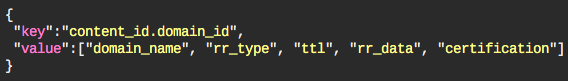
\includegraphics[scale=0.6]{figure/content-file.png}
 \caption{コンテンツのデータフォーマット}
 \label{fig:manager-provider}
\end{figure}

\hspace{-12pt}\textbf{フルサービスリゾルバ}\\
\hspace{12pt}フルサービスリゾルバは,サーバからの応答をキャッシュするを持つサービスノードである.
また,コンテンツIDおよびドメインIDを算出し,コンテンツを保持するマネージャに問い合わせる機能を担う.
全てのフルサービスリゾルバは,マネージャとそのマネージャのゾーンに関する対応表のファイルを保持している.
この対応表は,ICANNから提供される``Root.hints"ファイルのようにウェブ上で公開され,入手することができる.
フルサービスリゾルバは,アルゴリズム~\ref{algo:full-service}で示すように,スタブリゾルバからのクエリに含まれるドメイン名とレコードタイプに基づきコンテンツIDとドメインIDを導き出す.
コンテンツを保持するマネージャは,コンテンツIDが含まれるゾーンを探索することで一意に決定される.
名前解決には,``コンテンツID.ドメインID"のようにドット区切りでIDを組み合わせたものを識別子としてマネージャに問い合わせる.
レコード情報もしくは不在情報に関する応答パケットをマネージャから受け取ると,フルサービスリゾルバは既存システム同様に応答情報をキャッシュした後,スタブリゾルバに応答する.
\begin{table}[htb]
 \caption{フルサービスリゾルバが使用する関数と保持する情報}
 \centering
  \begin{tabular}{ll}
    \toprule
		\multicolumn{1}{c}{\textbf{表記}} & \multicolumn{1}{c}{\textbf{意味}} \\
    \midrule
		query\_manager() & マネージャに問い合わせる関数 \\
		response\_client() & 結果をクライアントに応答する関数 \\
		hash.sha3\_224() & 54bytesのSHA3ハッシュ関数 \\
    start & ゾーンにおける範囲の開始アドレス \\
    end & ゾーンにおける範囲の終了アドレス \\
    client\_address & クライアントのIPアドレスとポートのタプル \\
		answer.rcode & マネージャにおける応答コード \\
		answer.rdata & レコード情報 \\
    map\_start & ゾーンにおける範囲の開始アドレスのリスト \\
    map\_end & ゾーンにおける範囲の終了アドレスのリスト \\
    \bottomrule
  \end{tabular}
 \label{tab:discription-fullresolv}
\end{table}

\begin{algorithm}[htbp]
 \caption{フルサービスリゾルバにおける問い合わせ転送処理}
 \label{algo:full-service}
  \SetKwProg{Fn}{}{\string:}{}
  \SetKwFunction{Handle}{handler}
 $\vspace{-0.3cm}$\;
% クエリハンドリング\;
 \Fn{\Handle{query\_data,\ rtype}}{
   $content\_id,\ domain\_id \leftarrow calculate\_id(query\_data,\ rtype)$\;
	 $manager\_addr \leftarrow find\_manager(start,\ end,\ content\_id)$\;
	 $answer \leftarrow query\_manager(manager\_addr,\ content\_id,\ domain\_id)$\;
	 $response\_client(client\_address,\ qname,\ answer.rcode,\ answer.rdata)$\;
 }
 $\vspace{-0.3cm}$\;
\end{algorithm}


\newpage
\hspace{-12pt}\textbf{プロバイダ}\\
\hspace{12pt}プロバイダは,既存システムの権威サーバの機能のうち,レコード情報を操作する機能を担当するノードである.
すなわち,既存システムのSLD以降のドメイン情報に関して,作成・更新および消去といったレコード情報の操作を担当する.
メインの階層構造に上位のドメインを保持するマネージャが,プロバイダが保持するドメインのサーバ機能を担当する.
プロバイダは,認証局にてコンテンツ情報の真正性を評価されたのちに,プロバイダの上位に位置づくマネージャがそのコンテンツを担当するマネージャに依頼することでレコード情報を操作する.
プロバイダが認証局に転送する情報には以下の4つである.
\begin{itemize}
 \item ドメイン名
 \vspace{-3mm}
 \item レコードタイプ
 \vspace{-3mm}
 \item TTL(Time To Live)
 \vspace{-3mm}
 \item レコード情報
\end{itemize}
%%TTLの更新方法について説明する
%例えば,example.comプロバイダが``www"のIPアドレス情報を作成することを考える.
%example.comプロバイダは,``www.example.com"とレコードタイプ``A"およびその値``93.184.216.34"を含むデータを接続先のcomマネージャにリクエストする.
%comマネージャは,リクエストされたドメイン名とそれに関連づけるレコードタイプから識別子を算出し,担当のマネージャにストアリクエストを転送するという具合で動作する.

\newpage
\hspace{-12pt}\textbf{認証局}\\
\hspace{12pt}認証局は,レコード情報の真正性を検証する信頼された第3者機関である.
%目的から
DNSを用いた既存の名前解決システムでは,ドメイン名に任意の情報を関連づけることができることに起因して,DNSトンネリングとして利用される課題があった.
この課題に対してDNS-TDでは,ドメイン名に関連づけるレコード情報について,第3者機関からの認証を介在させることによって,不審な情報がドメイン名に関連づけられることを抑止する.
認証局を用いた認証プロセスでは,プロバイダからのドメイン名へのレコード情報を関連づけるリクエストをきっかけとする.
認証局に転送されるリクエストパケットについて,認証局は内容と依頼元の情報に基づいたデータの真正性を検証する.
この検証フェーズで認証されたコンテンツは,リクエストしたプロバイダの上位に位置づくマネージャに証明書を付与して転送される.
認証されなかった場合には,リクエストは破棄され,結果がリクエストしたプロバイダに応答される.

例えば,ドメイン名が``www.example.com"で,このドメイン名に``uname -ax"という文字列をTXTレコードに関連づけることを考える.
プロバイダは,認証局を宛先としてコンテンツの真正性に関する検証評価を依頼する.
依頼には,関連づける目的を合わせて要求する.
認証局は,関連づけたい内容と目的とを評価する.
この場合,``uname -ax"はLinuxコマンドであり不審なデータとして評価され,リクエストは破棄される.
関連づける情報が,IPアドレスであった場合には,接続性が評価された後,証明書を付与したコンテンツをマネージャに転送する.
これが認証における一連のプロセスであり,これによって不審なデータがドメインに関連づけられることを抑止する.
\begin{figure}[h]
 \centering
 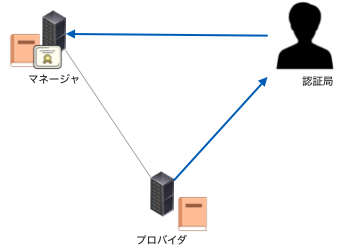
\includegraphics[scale=0.7]{figure/certificate-procedure.png}
 \caption{レコード情報操作におけるプロセスの概略図}
 \label{fig:manager-provider}
\end{figure}
% 認証局を導入するとインターネットの匿名性を実現することが難しくなるのではないか
% レコード情報に認証局を導入する場合,webなどのサービスやコンテンツを提供するのが少し困難になるではないかという懸念


\newpage
\subsection{識別子}
%ハッシュ空間によってIDが管理されることとどのハッシュ関数を使用するのかを説明する.
%ゾーンごとに分離される階層構造モデルに起因して発生するトンネリングに対して,フラットな名前構造が重要になる
本節では,コンテンツに付与する識別子について説明する.
DNSの名前解決システムでは,委譲の仕組みに基づいてドメインごとにゾーンを保持する設計のため,名前解決にあたりクエリ情報はそのドメイン名をゾーンとする権威サーバまで転送される.
この仕組みでは,ドメインを作成することで,そのドメインをゾーンにもつ権威サーバに対して任意の情報をDNSクエリに含めることでデータを転送することができる,DNSトンネリングとして機能する潜在的な特性がある.
転送する際に,正規のクエリ時に使用される長さや文字列に調整することで,正規クエリとトンネリングクエリを判別することは曖昧でき,このようにしてセキュリティシステムを迂回される脅威に発展する.
この課題は,名前空間を保持する機能とその空間上のドメイン情報を提供する機能が共在することに起因する.
そこで,DNS-TDでは,名前空間の保持機能と提供する機能を分離することで課題を解決する.
これは,ドメインの名前空間は維持したまま,コンテンツに識別子を付与し,この識別子の名前空間をフラットにすることで実現される.
DNS-TDでは,ドメイン名とレコードタイプという組みを単位として,全ての組みに画一的な名前空間上の値をその組みに識別子として付与する.
このように,DNS-TDでは,全てのドメイン名とレコードタイプの組みに識別子を付与するため,その識別子の名前空間は数の不足が無視できる程度に大きくなくてはならない.
また,~\ref{sec:stab-resolver}で述べるように,既存の名前解決の仕組みに依存したものは多く,プロトコルのフォーマットに変化を加えないことが望ましい.
DNSのクエリパケットにおいてデータを含められるQuestionセクションのQnameの最大長は,255bytesである.
また,Qnameはドメイン名を想定した設計になっているため,ドメイン名の制約にある最大63bytesとするラベル長の制約を満たす必要がある.
上記の制約を満たしながら,ドメイン名とレコードタイプから生成される識別子には,54bytesの名前空間を持つハッシュ関数によって生成されるメッセージダイジェストを用いる.
また,ダイジェストの衝突には,二重ハッシュ法に基づき対処する.
以降では,識別子に用いられるハッシュアルゴリズムとシステムの分散処理を目的としたゾーン分割法について説明する.

\subsubsection{ハッシュアルゴリズム}
本項では,コンテンツを識別するために使われる識別子の算出に利用するハッシュアルゴリズムについて説明する.
先に述べたように,提案システムで使用するハッシュアルゴリズムの要件は以下で示す通りである.
\begin{itemize}
 \item 不足を無視できる程度に大きい名前空間
 \vspace{-3mm}
 \item DNSプロトコルフォーマットへの準拠\\(ラベル長:最大63bytes,ドメイン長:最大253bytes)
\end{itemize}

%現在のインターネットにおいて,各権威サーバがゾーンを保持する設計のため,ドメイン名とレコードタイプの組みの数を正確に見積もることは困難である.
%ドメイン名の数は,インターネット上のサービスの数に相当すると考えることができ,そのドメイン名に関連づけられるリソースレコードの数は100も超えない数である.
%IPv6は全てのホストのインターフェースに一意に識別知を付与するのに,不足を無視できる名前空間として128bit(16bytes)を採用している.
%クライアントの数に比べて,サーバの数は少ないことは予想することができるが.その比率は不明である.
%そこで,現在使用できるハッシュアルゴリズムの特性から考える.
現在流布している代表的なハッシュアルゴリズムには,以下のようなものがある.
\begin{table}[htb]
 \caption{ハッシュアルゴリズムの一覧}
 \centering
  \begin{tabular}{lr}
    \toprule
		\multicolumn{1}{c}{\textbf{アルゴリズム}} & \multicolumn{1}{c}{\textbf{名前空間(bits)}} \\
    \midrule
		MD5 & 128 \\
		sha1 & 160 \\
		sha2 & 224,\ 256,\ 384,\ 512 \\
		sha3 & 224,\ 256,\ 384,\ 512 \\
    \bottomrule
  \end{tabular}
 \label{tab:hash-functions}
\end{table}

IPv6は全てのホストのインターフェースに一意に識別知を付与するのに,不足を無視できる名前空間として128bitsを採用している.
通常クライアント数の数に対してサーバの数は少なく,ドメイン名に関連づけられるリソースレコードの数はたかだか数から数十個である.
表~\ref{tab:hash-functions}で示すハッシュアルゴリズムの名前空間は,128bitsと同等かそれより大きい.
リソースレコードの数を含める
2のべき乗の桁数は,おおよそ$2^{0.301n}$$(n \in \mathbb{N})$から求めることできる.
で求めることができる.
これに基づき,160bitが

以上から,識別子として必要な名前空間は,128bitよりも少ない.
以上から,DNS-TDでは,最も出力長の短い56bytesの名前空間をもつsha3のアルゴリズムを採用する.

ハッシュ関数は有限空間に写像する性質から,写像したダイジェストが他のコンテンツによって算出されたダイジェストと衝突する可能性がある.
以降では,ダイジェストのコリジョンを回避するために,さらに名前空間は拡張するドメインIDについて説明する.
DNS-TDにおけるコンテンツIDは,ドメイン名とレコードタイプの文字列和をメッセージとするハッシュ関数のダイジェストである.

\begin{algorithm}[h]
 \caption{識別子の導出方法}
 \label{algo:calculate_id}
  \SetKwProg{Fn}{}{\string:}{}
  \SetKwFunction{Calc}{calculate\_id}
% $\vspace{-0.3cm}$\;
 \Fn{\Calc{qname, rtype}}{
   $content\_id \leftarrow hash.sha3\_224(qname+rtype)$\;
	 $domain\_id \leftarrow hash.sha3\_224(qname)[:28]$\;
	 $identity \leftarrow content\_id\ +\ ``."\ +\ domain\_id$\;
   $return \ identity$
 }
% $\vspace{-0.5cm}$\;
\end{algorithm}


例えば,ドメイン名が``www.example.com"でAのレコードタイプの組み合わせを考える.
アルゴリズム~\ref{algo:calculate_id}に従い,コンテンツIDのメッセージになるのは``www.example.comA"である.
そして,このメッセージをハッシュ関数にかけて算出された値``47d87[...中略...]4cb6"がコンテンツIDとなる.
ドメインIDは,ドメイン名をメッセージとするハッシュ関数から算出されるダイジェストの前半28bytesである.
すなわち,メッセージが``www.example.com"で,``86ff20[...中略...]bf026"がドメインIDとなる.
以上から,最終的なマネージャに問い合わせられる識別子は,それぞれのIDをドット区切りで連結された``(コンテンツID).(ドメインID)"となる.

\subsubsection{ゾーン分割}
本項では,ゾーンの分割方法とそのゾーンとマネージャの対応表について説明する.
DNS-TDにおけるゾーンは,ソートされたコンテンツIDの名前空間の連続した範囲に従って分割する.

\begin{table}[htb]
 \caption[マネージャとゾーンの対応表]{マネージャの情報とそのマネージャが管理するゾーンが記載された対応表の例}
 \centering
  \begin{tabular}{lrl}
    \toprule
		\multicolumn{1}{c}{\textbf{ゾーン}} & \begin{tabular}{c}\textbf{マネージャ}\\\textbf{アドレス}\end{tabular} & \multicolumn{1}{c}{\textbf{ドメイン}} \\
    \midrule
    (000…00, 2zz…zz) & 192.35.51.30 & com.  \\
		\multicolumn{1}{c}{...} & \multicolumn{1}{c}{...} & ... \\
    (500…00, 6zz…zz) & 192.5.6.30 & net. \\
		\multicolumn{1}{c}{...} & \multicolumn{1}{c}{...} & ... \\
    (b00…00, czz…zz) & 199.249.112.1 & org. \\
		\multicolumn{1}{c}{...} & \multicolumn{1}{c}{...} & ... \\
    (n00…00, mzz…zz) & 199.254.31.1 & info. \\
		\multicolumn{1}{c}{...} & \multicolumn{1}{c}{...} & ... \\
    (y00…00, zzz…zz) & 194.0.0.53 & arpa. \\
    \bottomrule
  \end{tabular}
 \label{tab:hash-management}
\end{table}


表~\ref{tab:hash-management}で示すように,``com"ドメインを管理するマネージャは``000...00"から``2xx...xx"の連続した範囲の名前空間を管理する.
コンテンツIDがこの範囲下に含まれる場合には,``com"に問い合わせることによってレコード情報を管理することができる.
対応表は,ICANNから提供される``Root.hints"ファイルのようにウェブ上で公開され,常時入手可能な状態が維持される.
全てのフルサービスリゾルバおよび認証局は,この対応表を保持することで,コンテンツIDを算出することで一意に管理するマネージャを特性することができる.

% 提案システムで使用するレコードタイプを概観するか,もしくは既存システムにおけるリソースレコードのタイプの課題から説明するのがいいだろう
\subsection{レコードタイプ}
本項では,DNS-TDで使用するリソースレコードのタイプについて説明する.
第~\ref{sec:dns-infiltration}項で示すように,既存の名前解決システムでドメインに関連づけることができるリソースレコードのいくつかのタイプは,DNS Infiltrationとして機能することができる.
DNS Infiltrationを抑止するリソースレコードであることの必要条件は,ドメインに関連のない任意の文字列がレコード情報に含められないことである.
既存のDNSのリソースレコードのタイプのうち,任意の文字列を含めることができるのタイプは以下の通りである.

表~\ref{tab:infil-rtype}のDNS Infiltrationとして機能する可能性のあるリソースレコードのタイプのうち,IPアドレスを偽装して情報を転送するものについては,第~\ref{sec:certificate}項で述べた認証基盤によってレコード情報の正当性評価で排除することができる.
NULL・TXT・CNAMEのレコードタイプも認証基盤における正当性の評価に基づいて,目的にそぐわない内容を含む場合には署名の作成を破棄することでDNS Infiltrationの発生を抑止する.

%特定のハッシュ範囲を管理するノードは,複数用意させ,そのアドレスを対応表に明記し,ストアする際にその全てのレプリケーションサーバにストアリクエストする
%DNSSEC~\cite{rfc4033}は,権威サーバからの応答パケットの偽装を検知することを目的として,データの作成元の確認とデータの完全性および,不在情報応答情報の証明するDNSの拡張仕様である.
%これは,主としてDNSの応答パケットを偽装できる程度のパラメータであることに起因する.
%他方で,DNS-TDでは,応答パケットに224bitのメッセージダイジェストが含まれるため,悪意のある応答パケットをフルサービスリゾルバに意図的にキャッシュすることは極めて困難である.以上の理由から,DNS-TDではDNSSECの目的にそぐわないため,リソースレコードとして使用されない.

